\documentclass{article}

\usepackage[english]{babel}
\usepackage[utf8]{inputenc}
\usepackage{amsmath,amssymb}
\usepackage{parskip}
\usepackage{graphicx}

% Margins
\usepackage[top=2.5cm, left=3cm, right=3cm, bottom=4.0cm]{geometry}
% Colour table cells
\usepackage[table]{xcolor}

\usepackage{hyperref}
\usepackage[english]{babel}

\usepackage[style=ieee]{biblatex}
\addbibresource{refs.bib}

% Get larger line spacing in table
\newcommand{\tablespace}{\\[1.25mm]}
\newcommand\Tstrut{\rule{0pt}{2.6ex}}         % = `top' strut
\newcommand\tstrut{\rule{0pt}{2.0ex}}         % = `top' strut
\newcommand\Bstrut{\rule[-0.9ex]{0pt}{0pt}}   % = `bottom' strut

%%%%%%%%%%%%%%%%%
%     Title     %
%%%%%%%%%%%%%%%%%
\title{Google Summer of Code 2021 \\ CODING PROJECT PROPOSAL \\ From DNA sequences to metabolic interactions: building a pipeline to extract key metabolic processes}

% \subtitle{CODING PROJECT PROPOSAL}
\author{
   \textbf{Name:} {Haris Zafeiropoulos} \\
   \textbf{Affiliation:} Department of Biology, University of Crete \\
   \textbf{Program:} PhD candidate, Second participation in GSoC \\
   \textbf{Mentors:} Elias Tsigaridas, Apostolos Chalkis, Zafeirakis Zafeirakopoulos \\
   \textbf{email:} \href{mailto:haris.zafr@gmail.com}{haris.zafr@gmail.com}\\
   \textbf{GitHub:} \href{https://github.com/hariszaf}{https://github.com/hariszaf}\\
   \textbf{Address:} Valestra 99, Heraklion, Crete, Greece, 71202\\
   \textbf{Phone:} +30 694 909 3089
}

\date{\today}

\begin{document}
\maketitle
\tableofcontents


%%%%%%%%%%%%%%%%%
%   Synopsis   %
%%%%%%%%%%%%%%%%%

\section{Synopsis}

Twenty years after Covert W.Covert, Bernhard O. Palsson and their colleagues published 
their review on metabolic modelling of microbial strains \cite{covert2001metabolic}, 
the value of this method has been well established. 

From the beginning, metabolic modeling has been interwoven with constraing-based methods \cite{palsson2015systems}. The value of randomized sampling in the framework of metabolic modeling has been proved itself over the years \cite{schellenberger2009use, herrmann2019flux}.

High Throughput Sequencing technologies have allowed process in the genetic information (DNA) in a cost-efficient and easy way, especially for microbial species as their genome is only but a few hundreds of genes long.

Once the complete genome of a species is obtained, the complete reconstruction of the metabolic network of the species is enabled, called genome-scale metabolic models (GEMs) \cite{gu2019current}.

Such models for all the species present in a microbial community, allows the study 
of metabolic interactions, thus an insight for the actual microbial intaractions \cite{ponomarova2015metabolic}. 

Aim of this project is to integrate the produced data and knowledge of these twenty 
(and more) years and make use of the randomized flux sampling method 
to evaluate the metabolic interactions retrieved. 
To this end, thousands of publicly available reference microbial genomes will be 
selected, and their automatic metabolic network reconstructions will be implemented. 
Based on these models, cross-feeding interactions algorithms will be performed for groups
of species to extract key metabolic processes. 
New functions, implementing the recently developed Multiphase Monte Carlo Sampling (MMCS) approach \cite{chalkis2020geometric} in the framework  of the \texttt{dingo} library, will 
make use of the randomized flux sampling concept to evaluate the processes retrieved.



%%%%%%%%%%%%%%%%%
% The project   %
%%%%%%%%%%%%%%%%%

\section{The Project}
\subsection{Background}
Microbial communities populate most environments on earth; from the seafloor to the
human gut, they literay live everywhere \cite{reise2009item}.
The play a critical role in shaping the environment as we know it.  
By driving biogeochemical cycles, 
bacteria, along with geochemical (abiotic) transformations (atmospheric, tectonic and geothermal), shape Earth's climate \cite{falkowski2008microbial}.
At the same time, *the human body is inhabited by millions of tiny living organisms* 
having a fundamental part in keeping us healty\cite{da2017we}. 
However, up to nowm scientists are able to cultivate approximately 1\% of known Bacteria \cite{tang2019microbial}. 
Since the growth of various bacteria depends on their interactions with others \cite{wade2002unculturable}, inferring microbial interactions would strongly support cultivating taxa for the first time, allowing the production of secondary metabolites and their biotechnological applications.
At the same time, it would be an essential tool to further expand our understanding
regarding the underlying mechanisms governing a range of phenomena, from ecosystem 
functioning to human health disorders.
This is why researchers from all these scientific fields have been studied the 
community structure of the microbial communities of their interest, 
focusing both on the taxa present and the metabolic processes (referred as *functions*). 

Metabolism is a network of the metabolic pathways that occur in an organism; thus, a metabolic network is the representation of all these pathways \cite{palsson2015systems}.
Using the stoichiometry of each reaction, which is always the same in the various species,
we convert the metabolic network of an organism into a mathematical model \cite{palsson2015systems}.
High Throughput Sequencing has made access to the complete genomic information of an organism rather easy. 
However, building the complete metbolic network of a species is not that trivial yet 
\cite{thiele2010protocol}.
However, over the last few years, automatic reconstruction approaches for building genome-scale metabolic models \cite{machado2018fast} of relatively high quality have been developed.

The study of metabolic dependencies to infer interspecies microbial interactions has been estrablished the last years (Fig.~\ref{interacting_community}), for more see \cite{zelezniak2015metabolic}.


\begin{figure}[h]
\label{interacting_community}
   \centering
   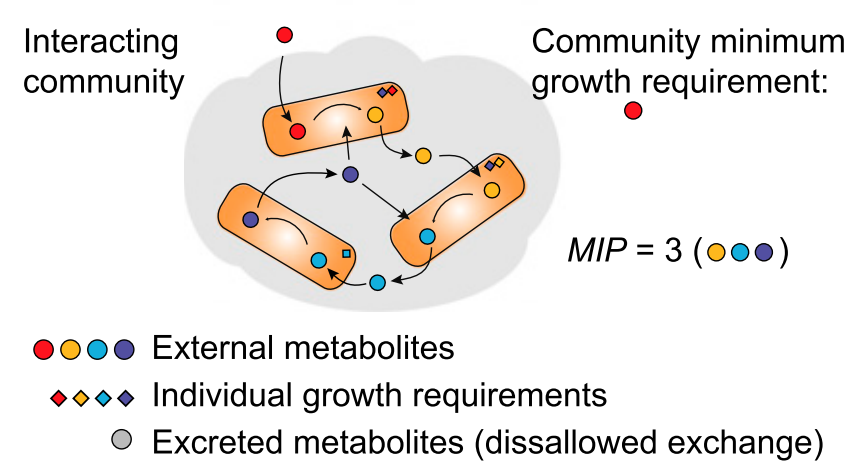
\includegraphics[width=0.8\textwidth]{interacting_community.png}
   \caption{Representation of a microbial community of 3 interacting species. 
   The Metabolic Interaction Potential metric (MIP) quatifies the propensity of a community to exhange metabolites. The figure is part of Fig. 3. at \cite{zelezniak2015metabolic}}
\end{figure}


Constrained-based modelling approaches, such as as Flux Balance Aanalysis and flux randomized sampling, have enabled the investigation of the properties of the possible steady states of a metabolic network,
end up with essential insights on metabolism at every level \cite{muller2018using, vieira2019comparison}.
Microbial communities harbor metabolically interdependent cooperative groups.
As a matter of fact, such groups play a key role for species co-occurrence \cite{zelezniak2015metabolic}.


The aim of this project is to bring together 
data (reference microbial genomes), 
automatic genome scale metabolic networks reconstruction tools,
cross-feeding interactions algorithms 
and flux randomized sampling.
This way, we will enable the evaluatation of the 
effect of each of the predicted metabolic interactions, 
to the various species of the community. 


\subsection{Methodology}
\label{methodology}
This project will make use of third party software tools and will also develop 
some new functions in the framework of the 
\href{https://github.com/GeomScale/dingo/}{\texttt{dingo}} project. 



\begin{figure}[h]
   \label{methods}
      \centering
      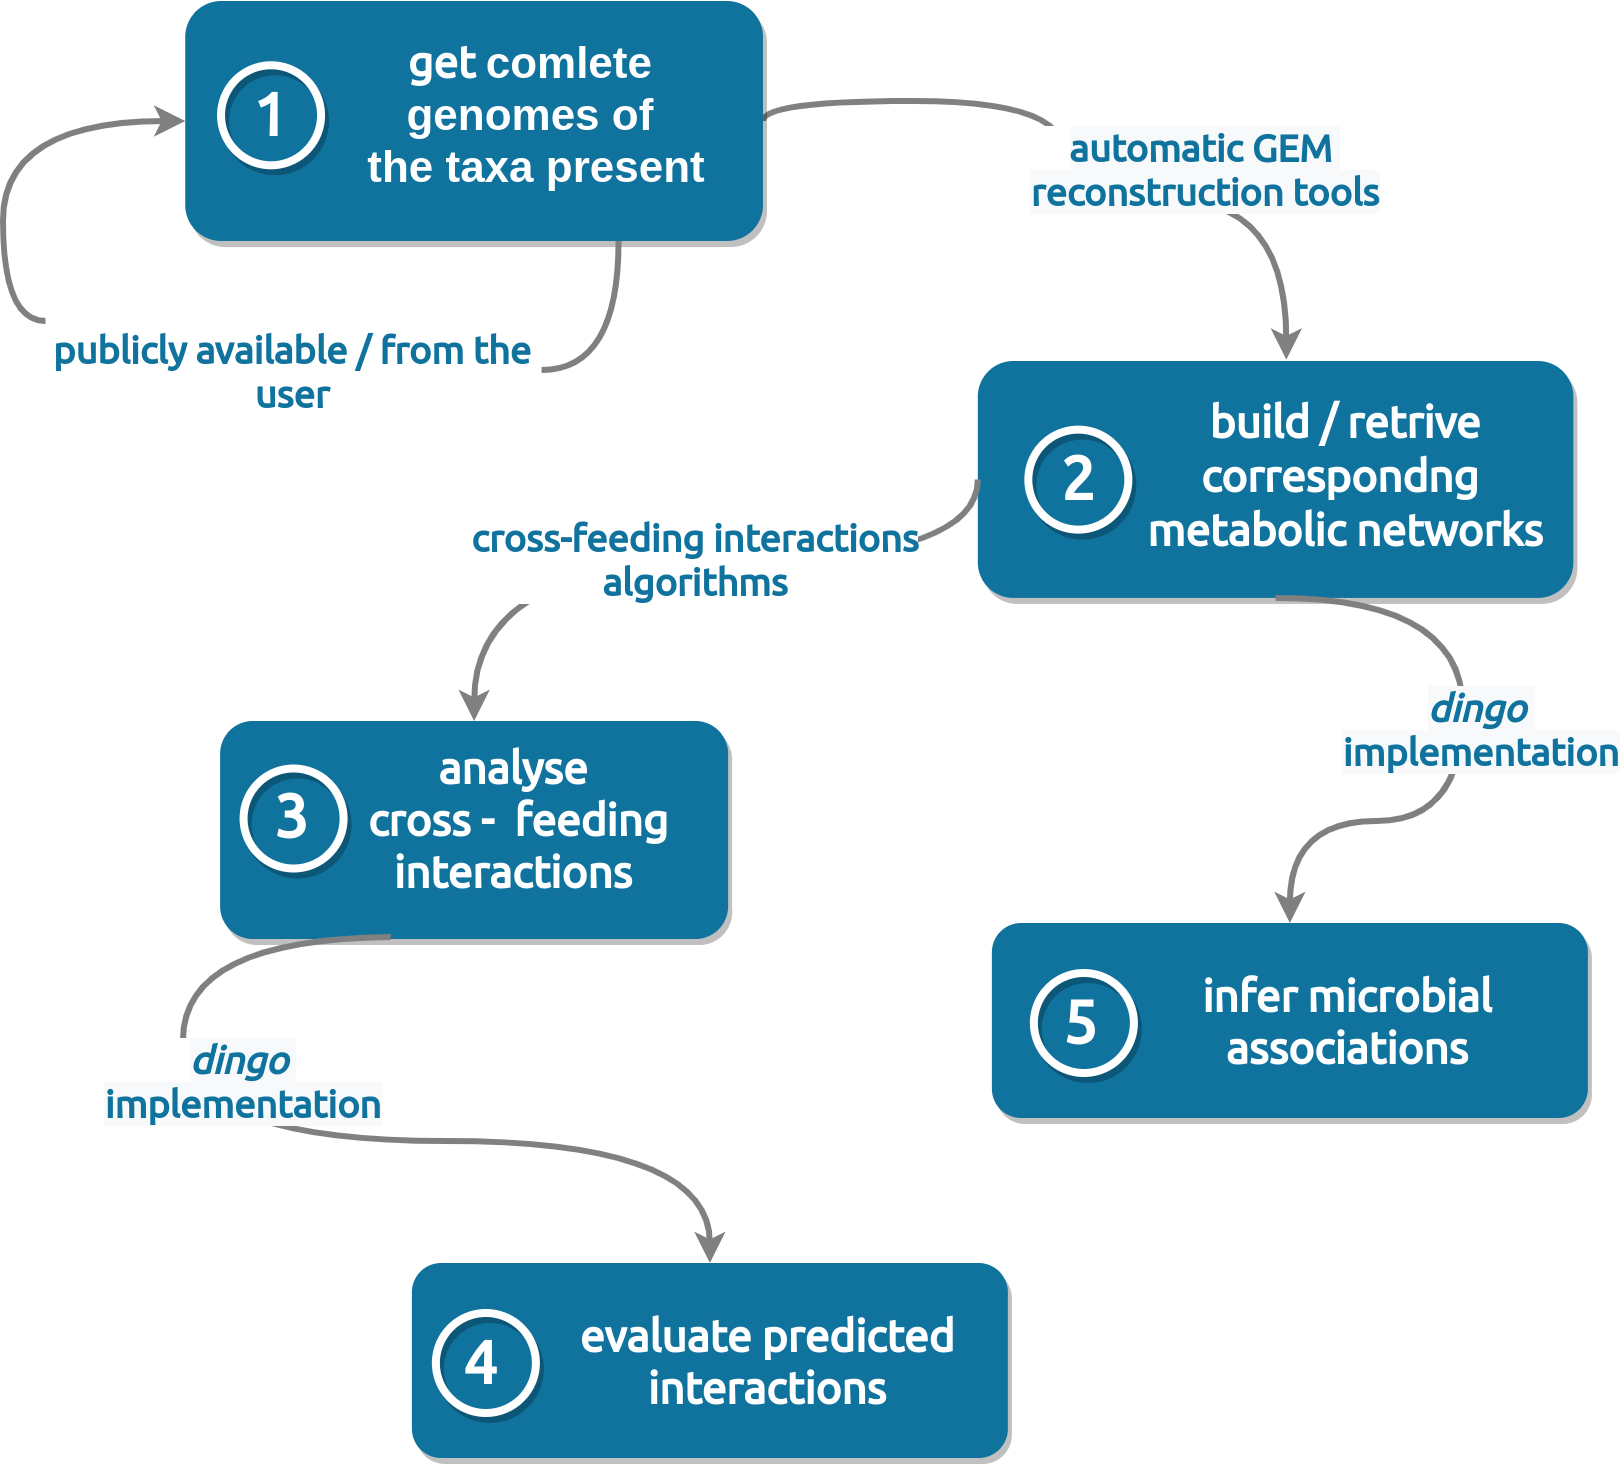
\includegraphics[width=0.8\textwidth]{proposal_fig.png}
      \caption{Project's workflow. This proposal consists of 4 major steps combining third party tools implementation and development of new code in the framework of the \texttt{dingo} Python library.}
\end{figure}



Global repositories including thousands of reference microbial genomes such as 
the Genome Taxonomy Database (GTDB) will be exploited \cite{parks2018standardized, parks2020complete}. 
% Here is a post on how to get the genomes of GTDB
% https://forum.gtdb.ecogenomic.org/t/194-600-genomes-r95-download/56 

Automatic genome scale metabolic networks reconstruction tools, 
such as AuReMe \cite{aite2018traceability} and CarveMe \cite{machado2018fast}, have been recently developed. Such tools will be implemented to get the corresponding GEMs 
for the genomes retrieved and/or for the genomed provided by the user. 

The \href{https://smetana.readthedocs.io/en/latest/algorithms.html}{SMETANA} package,
is a set of algorithms looking for possible cross-feeding interactions
between the species of the microbial community under study \cite{zelezniak2015metabolic}.
Such algorithms will be implemented in the GEMs built from the original genomes 
gathered or/and provided by the user, to return key metabolites. 

Flux randomized sampling using the MMCS algorithm of the \texttt{dingo} Python library 
will be implemented to evaluate the effect of the metabolites returned from the previous steps. 
To this end, new functions will be developed in the framework of the \texttt{dingo} library
to check the response of the biomass function \cite{feist2010biomass} or the function of maximization of ATP per unit flux \cite{schuetz2007systematic} in alterations regarding the corresponding metabolites. 
Furthermore, functions will be developed to perform sampling in the flux spaces of all the paired associations between the various species, to strengthen these associations, depending on whether they respond robustly on exchange/competition for metabolites. 


%%%%%%%%%%%%%%%%%
%    Benefits   %
%%%%%%%%%%%%%%%%%
\subsection{Benefits to the Community}

The proposed project will benefit the most the \texttt{dingo} Python library 
as an open source code project, as it will provide a thorough use case in a big-data scale and 
will also develop further functions for the analysis of microbial communities. 

Furthermore, it will be essential for biologists studying microbial interactions in all the different biological fields, from ecosystem functioning to precision medicine. 


%%%%%%%%%%%%%%%%%
% Deliverables  %
%%%%%%%%%%%%%%%%%
\section{Deliverables}
\subsection{Overview}
The tasks of this project will be split in the two main periods of the project; i.e. the Community Bonding period between the 17th of May to the 7th of June (~3 weeks) and the Coding period between the 7th of June and the 16th of August (~10 weeks). 
At the end of the coding period, all the implementations described in the Deliverables described above, will have been completed. 

The \texttt{dingo} library provides a great basis for the implementation of this project. 
Therefore, a limited amount of time is needed  to set up all the necessary coding environments. 
As I have been involved with the GeomScale group and the \texttt{dingo} library for over a year, it will not need time to get used to the group's working framework.
In addition, the proposed subject has been discussed and thorough study of the 
scientific issues that might occur, will be addressed before the bonding period starts.

That said, the coding tasks could start before the bonding period is over. 
Furthermore, a blog will be created to report the project’s progress periodically and a thorough documentation for the \texttt{dingo} Python library will be delivered
as well as a repository with the models built.

The \texttt{dingo} library is under the LGPL-3 license. 
However, as the workflow will make use of third-party tools separate licenses will apply.



\subsection{Bonding period (May 17 - June 7)}
Main milestone of the bonding period will be to communicate with biologists 
to address and confirm all the scientific-oriented issues that might occur. 
A group of molecular ecologists have already knowledge of the project and I will be in 
contact with them even before bonding period starts. 

The first two weeks will require a strong effort from me 
in designing, the \texttt{dingo} functions as well as the setup of
the repository for the models that will be about to build and 
the download/storage of their corresponding genomes. 
The mentors’ guidance will be essential during this time. 

In the third week of the bonding period, it is my intention to be ready to start coding. 
I do not count it as a coding week, however I believe I will be ready.

Furthermore, I will build a \texttt{git} branch from the \texttt{dingo} GitHub repository
and a blog to report my progress periodically.




\subsection{Coding period (June 7 - August 16)}

This 10 weeks period will be split in the following time windows, each of which corresponds to a certain milestone: 


\textbullet\ \textbf{Weeks: \#1 and \#2}
% leave next line empty on purpose

In the first 2 weeks, the repository where the genomes and the models will be stored will be built, Fig.~\ref{methods} box 1. 
In addition, the more than 190,000 genomes from the GTDB will be downloaded. 
A deamon for getting new or updated genomes will be also set.
A first documentation of the repository and how to access it will be delivered.

\textbullet\ \textbf{Week: \#3}
% leave next line empty on purpose

In this week, the two software tools mentioned in the~\pageref{methodology} section for automatic GEM reconstruction, will be thoroughly tested and it will be decided which 
will be used, Fig.~\ref{methods} box 2. 
GEMs then will be built and stored. 
Format-oriented issues will be also addressed.  
The models built during this week will be available via the blog of the project as well. 

\textbullet\ \textbf{Weeks: \#4 to \#7}
% leave next line empty on purpose

During this period, the SMETANA algorithms will be implmemented for all the models built by that time. 
Thourough examination of the output will be performed Fig.~\ref{methods} box 3. 
Once a small number of successful runs of the SMETANA algorithms are completed, I 
will start developing the \texttt{dingo} functions for the evaluation of the metabolities returned, Fig.~\ref{methods} box 4. 
As this will be the most complicated task, both from the coding and the biology point of view, 
extensive communication both with the mentors of the project and biologists will be held 
to its fine completion. 
A short report with the process of the project during this period will be delivered in the project's blog.


\textbullet\ \textbf{Weeks: \#8 and \#9}
% leave next line empty on purpose

In those two weeks, \texttt{dingo} functions for inferring microbial interactions 
in pairs of GEMs will be developed, Fig.~\ref{methods} box 5. 
Just like the previous milestone, this part will be developed side-by-side with 
biologists ensuring that the new functions developed, provide valid outcome. 
As this part is rather scientific, if further developments is needed, I will discuss this 
with the mentors to continue working on that even after the project is complete. 
By the end of this period, I will have a report delivered in the project's blog.


\textbullet\ \textbf{Week: \#10}
% leave next line empty on purpose

During this last week, tests for the complete pipeline will be held. 
Thourough documentation for the pipeline will be provided. 
I will make a Pull Request, so my branch to merge with the \texttt{main} branch of the \texttt{dingo} library. 
I will finally submit the final evaluation of the GSoC project.


\rule{\textwidth}{0.4pt}

\textbf{Comment:} The above time schedule is a worst-case schedule. 
However, if the coding exceeds my present expectations I will discuss with mentors new additions and implementations.

There are not schedule conflicts during the summer. 

\rule{\textwidth}{0.5pt}

%%%%%%%%%%%%%%%%%
% Related work  %
%%%%%%%%%%%%%%%%%
\section{Related work}

I have been a member of the GeomScale project over the last year.
Based on \href{https://github.com/GeomScale/gsoc2020/wiki/High-dimensional-sampling-with-applications-to-structural-biology}{an idea from the GSoC of 2020} we have been working on sampling the flux space of metabolic networks. 
I contributed with wrapping the C++ code of \texttt{VolEsti} to build the Python interface.
Furthermore, I implemented the MMCS method developed by the GeomScale group on metabolic networks of high dimensions \cite{chalkis2020geometric}. 
This work was accepted in the proceedings of the \href{https://cse.buffalo.edu/socg21/accepted.html}{37th Symposium on Computational Geometry}.



%%%%%%%%%%%%%%%%%
%     Tests     %
%%%%%%%%%%%%%%%%%
\section{Tests}
This proposal is not among the ideas listed in the 
\href{https://github.com/GeomScale/gsoc2021/wiki/table-of-proposed-coding-projects}{table of proposed coding projects} of the GeomScale group. 
As the scope of my proposal is close to the \href{https://github.com/GeomScale/gsoc2021/wiki/Inferring-microbial-interactions}{Inferring microbial interactions} project, 
and after contacting the mentors, 
I implemented the tests of the latter project in the framework of my proposal.

You can find my answers on this \href{https://hariszaf.github.io/gsoc2021/}{link} 
and the correspondig code on its correspondig \href{https://github.com/hariszaf/gsoc2021}{GitHub repository}.



%%%%%%%%%%%%%%%%%
%      CV       %
%%%%%%%%%%%%%%%%%
\section{Biographical information}
\subsection{Education}

\begin{itemize}

   \item PhD candidate at University of Crete (2018 - ongoing). Dissertation on: “Merging NGS data, knowledge aggregation and data integration techniques, along with ecological network analysis (ENA): an attempt to decipher microbial community ecology and ecosystem functioning by taking advantage of the hypothesis-generating method”.
   \item MSc in Bioinformatics at the University of Crete (2016 - 2018). Thesis: “eDNA metabarcoding for biodiversity assessment: Algorithm design and bioinformatics analysis pipeline implementation”
   \item BSc in Biology at the National and Kapodistrian University of Athens (2010 - 2016). Thesis: “Morphology, morphometry and anatomy of species of the genus Pseudamnicola in Greece” 

\end{itemize}


\subsection{Publications}

\begin{itemize}

   \item Zafeiropoulos, Haris, Anastasia Gioti et al. 0s and 1s in marine molecular research: a regional HPC perspective (\textbf{under review in GigaScience journal})

   \item Zafeiropoulos, Haris, Anastasia Gioti et al. (2021, April 5). The IMBBC HPC facility: history, configuration, usage statistics and related activities (Version 1.0.0). Zenodo. DOI: \href{http://doi.org/10.5281/zenodo.4665308}{10.5281/zenodo.4665308}

   \item Polymenakou, Paraskevi N., et al. "The Santorini Volcanic Complex as a Valuable Source of Enzymes for Bioenergy." Energies 14.5 (2021): 1414. DOI: \href{https://doi.org/10.3390/en14051414}{10.3390/en14051414}
   
   \item Chalkis, Apostolos, et al. "Geometric algorithms for sampling the flux space of metabolic networks." arXiv preprint arXiv:2012.05503 (2020) \href{https://hal.inria.fr/hal-03047049v2}{https://hal.inria.fr/hal-03047049v2}
   
   \item Zafeiropoulos, Haris, et al. "PEMA: a flexible Pipeline for Environmental DNA Metabarcoding Analysis of the 16S/18S ribosomal RNA, ITS, and COI marker genes." GigaScience 9.3 (2020): giaa022.. 
   DOI:\href{https://doi.org/10.1093/gigascience/giaa022}{10.1093/gigascience/giaa022}
   
\end{itemize}


\subsection{Programming}

\begin{itemize}
   \item Author of the \href{https://github.com/hariszaf/pema}{\texttt{PEMA}} workflow
   \item Very experienced in programming with scripting programming languages \\
   (Python, BigDataScript, R).
   \item Basic knowledge of C++
   \item Very experienced in container-based technologies (Docker, Singularity)
   \item Experienced in web 
\end{itemize}


\subsection{Personal motivation}

Bioinformatics play a great part in almost every aspect of modern biology.
Metabolic interactions \cite{cai2020predicting} is now the next big thing in systems biology. 
That is why after graduating Biology school (BSc), I focused on computer science and Bioinformatics (MSc). 
I am now quite experienced with a series of scripting programming languages (Python, BigDataScript, R) and with container-based technologies (Docker, Singularity).  
% PEMA \cite{zafeiropoulos2020pema}, a pipeline for the analysis of metabarcoding data, was my first coding project; PEMA has now been published and selected from \href{https://www.lifewatch.eu/}{LifeWatch - ERIC} a European Researh Infrustructure, to support .
% \href{http://prego.hcmr.gr/}{PREGO} and \href{https://github.com/hariszaf/darn/}{DARN} are ongoing bioinformatics projects in the framework of my PhD.


My research interests focus on ecology and ecosystem functioning at the microbial dimension.
As Systems Biology approaches can benefit the most this field, 
I have spent the last 2 years working on 
knowledge aggregation and data integration techniques as well as networks analysis are employed. 
Metabolic interactions \cite{cai2020predicting} is now the next big thing in systems biology. 
Over the last year, I have been working with the GeomScale group on the \href{https://github.com/GeomScale/volume_approximation}{\texttt{VolEstipy}} project.
Developing algorithms for sampling on the flux space of metabolic networks have 
helped me in getting a more holistic point of view of the potentials of sampling in the study of metabolic networks. 

This GSoC project would allow me to continue working with the GeomScale group, 
whilst building the proposed application would benefit me the most, 
especially as it will allow me to extend the scopus of my PhD dissertation.

% In such a study, the changing phenotype of an ecosystem, as derived by the combination of phenotypes of all the ecosystem's individual entities, under different scenarios of constraint values could be predicted. 
% The impact of such studies would be more than significant, especially on a time when nature suffers the most, mostly due to anthropogenic activities. 
% Indicatively possible datasets such a study could be conducted on: 
% “Impact of exogenous nitrogen on the cyanobacterial abundance and community in oil-contaminated sediment: A microcosm study” from Wang et al. [19] 
% (peer-reviewed, no public data, email request)
% “Discovery of functional gene markers of bacteria for monitoring hydrocarbon pollution in the marine environment - a metatranscriptomics approach” from Knapik et al. [20]
% (not peer-reviewed, data not published yet)
% In their study [21], Gossart et al.  describe the research framework of such studies we suggest to apply the aforementioned methods .


% Coding has been a great part of my everyday routine through the recent years. 
% The different needs of the different types of analysis in biology force you to deal with a great range of computing tasks, such as choosing the proper programming language for each issue, working with High Performance Computing environments, finding ways to make your code easy-to-use, easy-to-distribute and flexible at the same time. 
% It would be both a profit and an enjoyment for me to be part of the Google Summer of Code and upgrade my so-far programming skills, particularly as \texttt{dingo} functions have been developed in C++, meaning that I will have to deal with new personal coding challenges. 




%%%%%%%%%%%%%%%%%
%   add REFS    %
%%%%%%%%%%%%%%%%%

\printbibliography

\end{document}
